\chapter{El telescopio de muones MuTe}
\label{Cap:MuTe}
El proyecto MuTe\footnote{https://halley.uis.edu.co/fuego} busca diseñar, construir, calibrar y poner en funcionamiento un telescopio que permita aplicar la muongrafía a volcanes en Colombia para generar perfiles de densidad y determinar la estructura interna de la zona central de los mismos. MuTe se compone de dos detectores: un detector Cherenkov de agua (WCD) y un hodoscopio de centelladores plásticos como se muestra en la fig. \ref{fig:MuTe}.\\ \\
El WCD permite detectar la radiación Cherenkov producida por el paso de partículas cargadas con una velocidad mayor a la velocidad de la luz en el agua. Se utiliza para identificar si la partícula incidente pertenece a la componente muónica del flujo de secundarios \citep{Tesis_adriana}.
\begin{figure}[h!]
\begin{centering}
  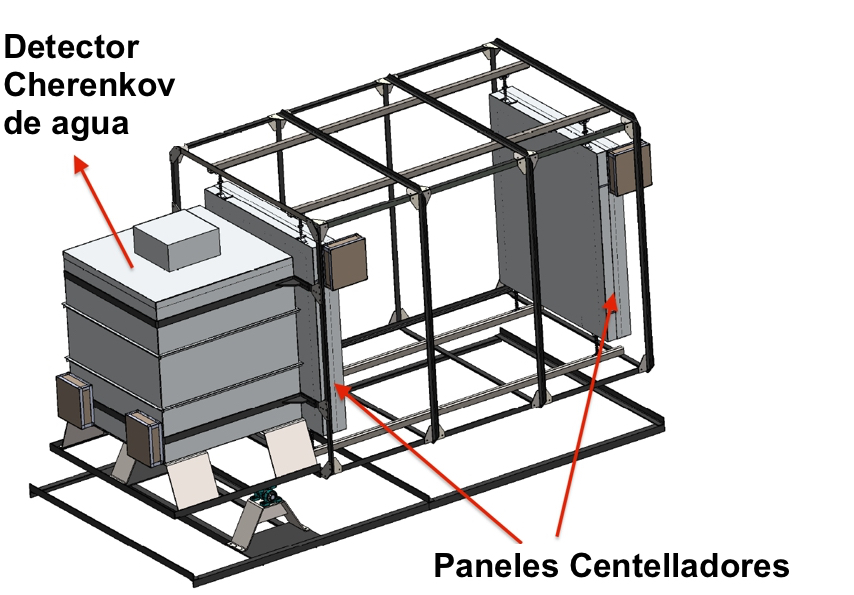
\includegraphics[width=0.75\textwidth]{Images/Mute.JPG}
  \caption{Telescopio de muones (MuTe), diseñado para la muongrafía de volcanes en Colombia, compuesto por un detector Cherencov de agua y dos paneles centelladores que configuran un hodoscopio. Adaptado de \citep{MuTe_mec}.}
  \label{fig:MuTe}
  \par\end{centering}
\end{figure}
\\ \\
Por otra parte, como se muestra en la figura \ref{fig:Hodoscopio} el hodoscopio está compuesto por dos paneles centelladores que permiten determinar la dirección de las partículas cargadas provenientes del volcán. En cada panel están ubicadas 30 barras centelladoras horizontales y 30 verticales. El material plástico de los centelladores genera fotones  cuando una partícula cargada lo atraviesa, estos fotones son guiados por una fibra óptica de corrimiento de longitud de onda (WLS) hasta el dispositivo sensor.    
\begin{figure}[h!]
\begin{centering}
  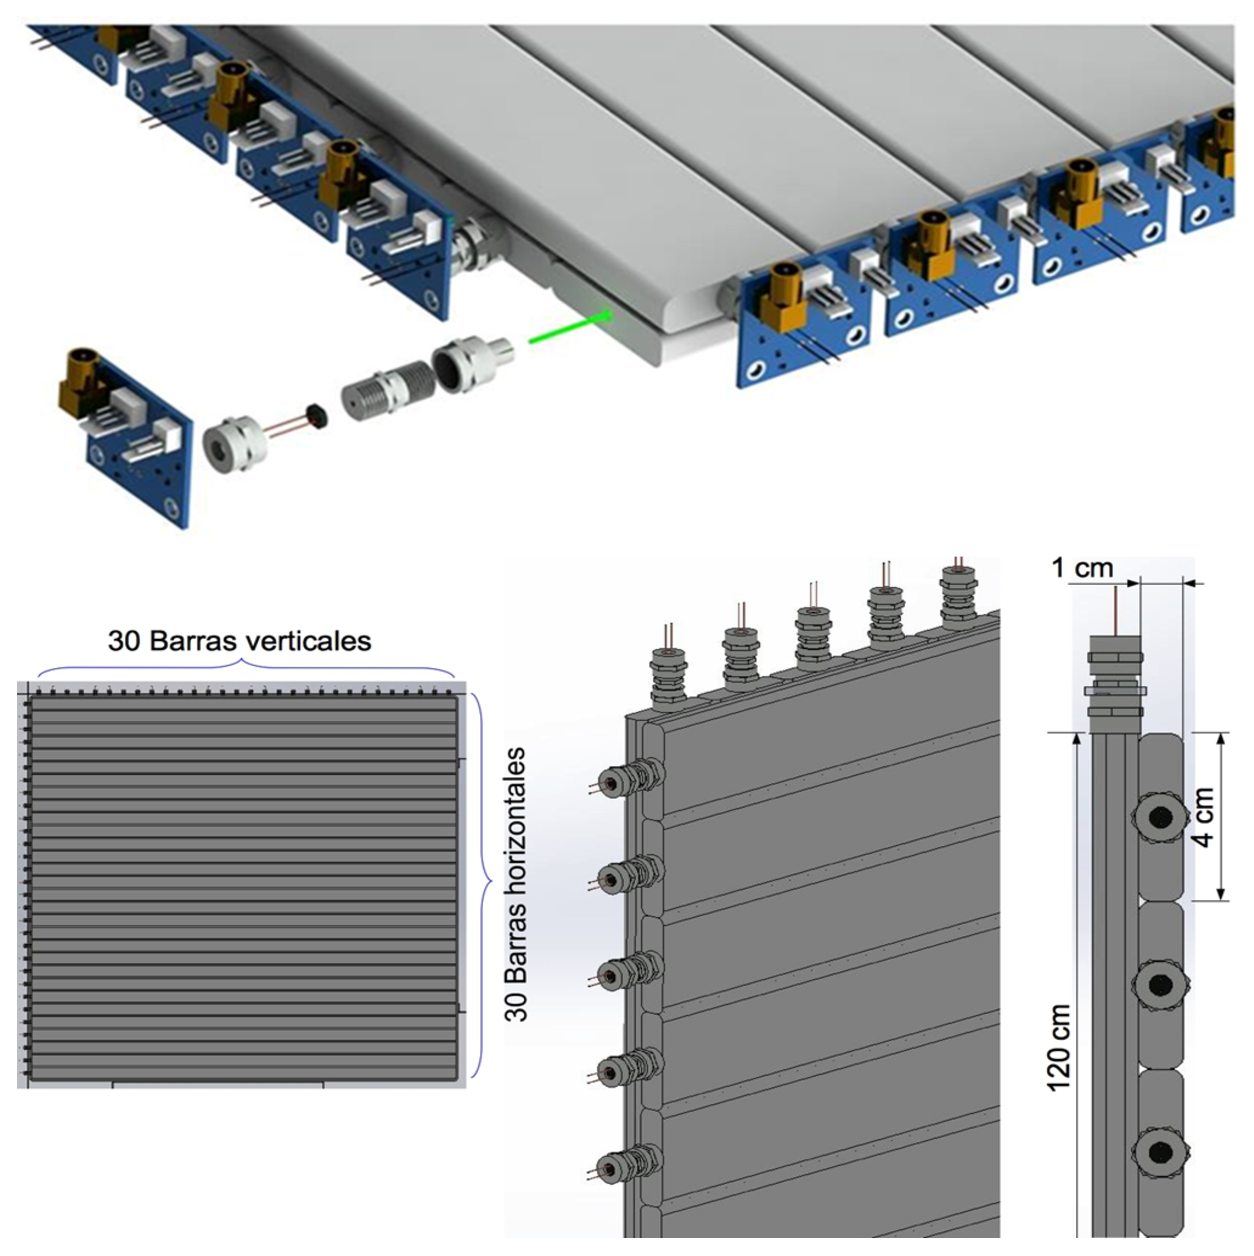
\includegraphics[width=0.55\textwidth]{Images/Panel.eps}
  \caption{Paneles centelladores del MuTe, cada una de las barras que componen el panel tiene acoplado un SiPM en un extremo, junto a una tarjeta electrónica con una etapa de amplificación. Adaptado de \citep{MuTe_mec}.}
  \label{fig:Hodoscopio}
  \par\end{centering}
\end{figure}